% ------------------------------------------------------------------------------
% TYPO3 CMS 8.6 - What's New - Chapter "Introduction" (French Version)
%
% @author	Michael Schams <schams.net>
% @license	Creative Commons BY-NC-SA 3.0
% @link		http://typo3.org/download/release-notes/whats-new/
% @language	French
% ------------------------------------------------------------------------------
% LTXE-CHAPTER-UID:		7fdf26cc-362160ab-d6c8b905-19722b20
% LTXE-CHAPTER-NAME:	Introduction
% ------------------------------------------------------------------------------

\section{Introduction}
\begin{frame}[fragile]
	\frametitle{Introduction}

	\begin{center}\huge{Introduction}\end{center}
	\begin{center}\huge{\color{typo3darkgrey}\textbf{Faits}}\end{center}

\end{frame}

% ------------------------------------------------------------------------------
% LTXE-SLIDE-START
% LTXE-SLIDE-UID:		b088f6b9-9942d4d1-026567a3-bd110d43
% LTXE-SLIDE-ORIGIN:	ea30ee1a-0bc39e0a-bcaf8d4b-fccc3d18 English
% LTXE-SLIDE-TITLE:		TYPO3 CMS 8.6 - The Facts
% ------------------------------------------------------------------------------
\begin{frame}[fragile]
	\frametitle{Introduction}
	\framesubtitle{TYPO3 CMS 8.6 - Faits}

	\begin{itemize}
		\item Date de sortie~: 14 février 2017
		\item Type de sortie~: Sprint Release
		\item Slogan~: «~Polishing~»
	\end{itemize}

	\begin{figure}
		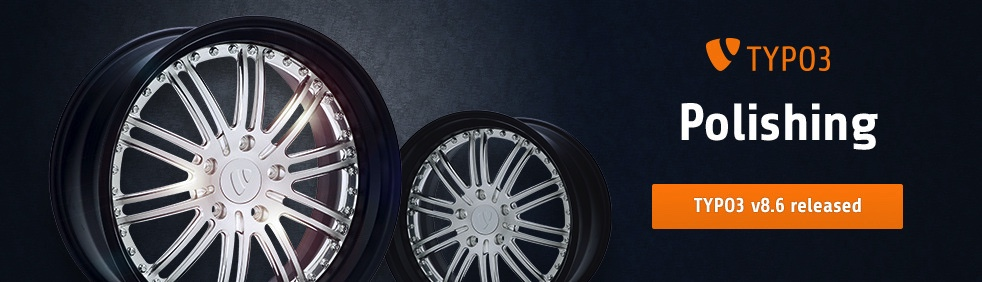
\includegraphics[width=0.95\linewidth]{Introduction/typo3cms86-banner.jpg}
	\end{figure}

\end{frame}

% ------------------------------------------------------------------------------
% LTXE-SLIDE-START
% LTXE-SLIDE-UID:		068bb408-96c47690-d42ce091-557d092b
% LTXE-SLIDE-ORIGIN:	edf38742-589c1a34-ae855361-e0284741 English
% LTXE-SLIDE-TITLE:		System Requirements
% ------------------------------------------------------------------------------
\begin{frame}[fragile]
	\frametitle{Introduction}
	\framesubtitle{Prérequis système}

	\begin{itemize}
		\item PHP~:\tabto{2.5cm}version 7
		\item MySQL~:\tabto{2.5cm}version 5.5 à 5.7
		\item Espace disque~:\tabto{2.5cm}min. 200 Mo
		\item Configuration PHP~:

			\begin{itemize}
				\item \texttt{memory\_limit} >= 128M
				\item \texttt{max\_execution\_time} >= 240s
				\item \texttt{max\_input\_vars} >= 1500
				\item L'option de compilation \texttt{-}\texttt{-disable-ipv6} \underline{NE} doit \underline{PAS} être utilisée
			\end{itemize}

		\item Le backend nécessite Microsoft Internet Explorer 11 ou ultérieur,
			Microsoft Edge, Google Chrome, Firefox, Safari ou tout autre navigateur
			moderne compatible

	\end{itemize}

\end{frame}

% ------------------------------------------------------------------------------
% LTXE-SLIDE-START
% LTXE-SLIDE-UID:		d8287b21-e9a2ea1e-66990183-cfe37018
% LTXE-SLIDE-ORIGIN:	8cb2705f-d045b3fa-b2ca4f81-52d16aef English
% LTXE-SLIDE-TITLE:		Development And Release Timeline
% ------------------------------------------------------------------------------
\begin{frame}[fragile]
	\frametitle{Introduction}
	\framesubtitle{Chronologie des développements et sorties}

	\begin{figure}
		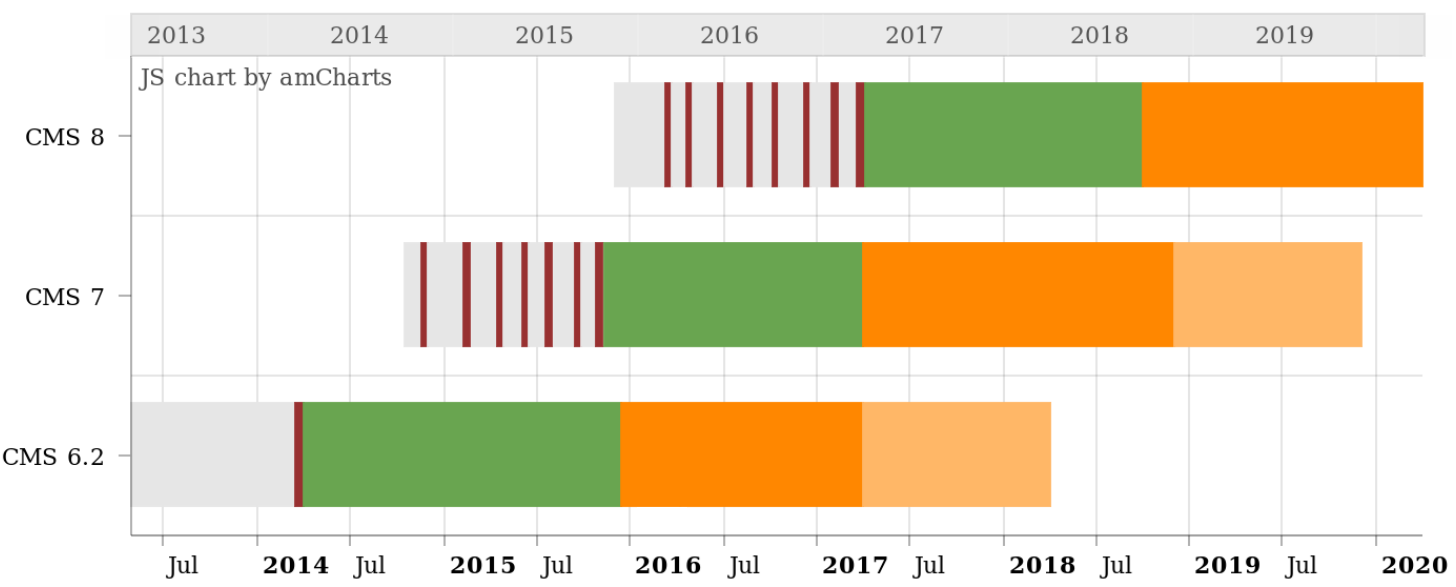
\includegraphics[width=1\linewidth]{Introduction/ReleaseAgenda.png}
	\end{figure}

\end{frame}

% ------------------------------------------------------------------------------
% LTXE-SLIDE-START
% LTXE-SLIDE-UID:		323d0e1a-421aa511-a4529c3b-c7f1b22c
% LTXE-SLIDE-ORIGIN:	dae3f732-e4550c37-dc304056-f090affc English
% LTXE-SLIDE-TITLE:		TYPO3 CMS Roadmap
% ------------------------------------------------------------------------------
\begin{frame}[fragile]
	\frametitle{Introduction}
	\framesubtitle{Feuille de route TYPO3 CMS}

	Dates de sortie et axes principaux~:

	\begin{itemize}

		\item v8.0 \tabto{1.1cm}22/Mars/2016\tabto{3.4cm}Adding last minute things
		\item v8.1 \tabto{1.1cm}03/Mai /2016\tabto{3.4cm}Cloud Integration
		\item v8.2 \tabto{1.1cm}05/Jui./2016\tabto{3.4cm}Doctrine Prerequisites
		\item v8.3 \tabto{1.1cm}30/Août/2016\tabto{3.4cm}Rich Text Editor
		\item v8.4 \tabto{1.1cm}18/Oct./2016\tabto{3.4cm}Doctrine Migration + Upgrades
		\item v8.5 \tabto{1.1cm}20/Déc./2016\tabto{3.4cm}New RTE + Integrator Support
		\item
			\begingroup
				\color{typo3orange}
					v8.6 \tabto{1.1cm}14/Fév./2017\tabto{3.4cm}Polishing
			\endgroup
		\item v8.7 \tabto{1.1cm}04/Avr./2017\tabto{3.4cm}LTS Preparation

	\end{itemize}

	\smaller
		\url{https://typo3.org/typo3-cms/roadmap/}\newline
		\url{https://typo3.org/news/article/kicking-off-typo3-v8-development/}
	\normalsize

\end{frame}

% ------------------------------------------------------------------------------
% LTXE-SLIDE-START
% LTXE-SLIDE-UID:		eb7ef89c-f087fc94-5222c387-67bda8fb
% LTXE-SLIDE-ORIGIN:	4a382358-6fd84263-041bc029-bd50bb1e English
% LTXE-SLIDE-TITLE:		Installation
% ------------------------------------------------------------------------------
\begin{frame}[fragile]
	\frametitle{Introduction}
	\framesubtitle{Installation}

	\begin{itemize}
		\item Procédure officielle \textit{classique} d'installation sous Linux/Mac OS X\newline
			(DocumentRoot considéré \texttt{/var/www/site/htdocs})~:
		\begin{lstlisting}
			$ cd /var/www/site
			$ wget --content-disposition get.typo3.org/8.6
			$ tar xzf typo3_src-8.6.0.tar.gz
			$ cd htdocs
			$ ln -s ../typo3_src-8.6.0 typo3_src
			$ ln -s typo3_src/index.php
			$ ln -s typo3_src/typo3
			$ touch FIRST_INSTALL
		\end{lstlisting}

		\item Liens symboliques sous Microsoft Windows~:

			\begin{itemize}
				\item Utiliser \texttt{junction} sous Windows XP/2000
				\item Utiliser \texttt{mklink} sous Windows Vista et Windows 7
			\end{itemize}

	\end{itemize}
\end{frame}

% ------------------------------------------------------------------------------
% LTXE-SLIDE-START
% LTXE-SLIDE-UID:		b8fce37f-8b0bcfdc-c0d851bb-ff95e431
% LTXE-SLIDE-ORIGIN:	db02b644-4eae727a-2eff0fa0-9cbd7fd3 English
% LTXE-SLIDE-TITLE:		Upgrade to TYPO3 CMS 7
% ------------------------------------------------------------------------------
\begin{frame}[fragile]
	\frametitle{Introduction}
	\framesubtitle{Mise à jour vers TYPO3 CMS 8.x}

	\begin{itemize}
		\item Les mises à jour sont possibles seulement depuis TYPO3 CMS 7.6 LTS
		\item TYPO3 CMS < 7.6 LTS doivent être mis à jour vers la 7.6 LTS en premier
	\end{itemize}

	\begin{itemize}

		\item Instructions de mise à jour~:\newline
			\smaller\url{http://wiki.typo3.org/Upgrade#Upgrading_to_8.6}\normalsize
		\item Guide TYPO3 officiel «~TYPO3 Installation and Upgrading~»~:
			\smaller\url{http://docs.typo3.org/typo3cms/InstallationGuide}\normalsize
		\item De manière générale~:
			\begin{itemize}
				\item Vérifier les prérequis système \small(PHP, MySQL, etc.)
				\item Examiner \textbf{deprecation\_*.log} de l'ancienne instance TYPO3
				\item Mettre à jour toutes les extensions vers leurs dernières versions
				\item Déployer les nouvelles sources et exécuter l'assistant de mise à jour de l'Install Tool
				\item Examiner le module de démarrage des utilisateurs backend (optionnel)
			\end{itemize}
	\end{itemize}

\end{frame}

% ------------------------------------------------------------------------------

% ------------------------------------------------------------------------------
% LTXE-SLIDE-START
% LTXE-SLIDE-UID:		c17d3a19-e63859a9-fe99ab7e-723ad2f4
% LTXE-SLIDE-ORIGIN:	d9a72263-ac0c63dd-1754b138-99b8491c English
% LTXE-SLIDE-TITLE:		PHP Version 7
% ------------------------------------------------------------------------------
\begin{frame}[fragile]
	\frametitle{Introduction}
	\framesubtitle{PHP Version 7}

	\begin{itemize}

		\item PHP 7.0 est le prérequis minimum pour TYPO3 CMS 8.x
		\item TYPO3 supportera les sorties de PHP 7 au fur et à mesure
		\item Cette montée de version apporte une amélioration
			significative des performances de l'ensemble du système

		\item Non seulement les éditeurs backend remarquerons une interface plus fluide,
			mais le nouveau record de chargement d'une page entièrement en cache en
			frontend est sous les 7 millisecondes, approximativement 40\% plus rapide
			que le même site avec PHP version 5.5

		\item Nous avons aussi commencé à utiliser les nouvelles fonctionnalités de cette version,
			par exemple les générateurs pseudo-aléatoires sécurisés cryptographiquement sont
			déjà utilisés. (Cryptographically secure pseudorandom number generator~; CSPRNG)

	\end{itemize}

\end{frame}

% ------------------------------------------------------------------------------
